\begin{figure}
\centering
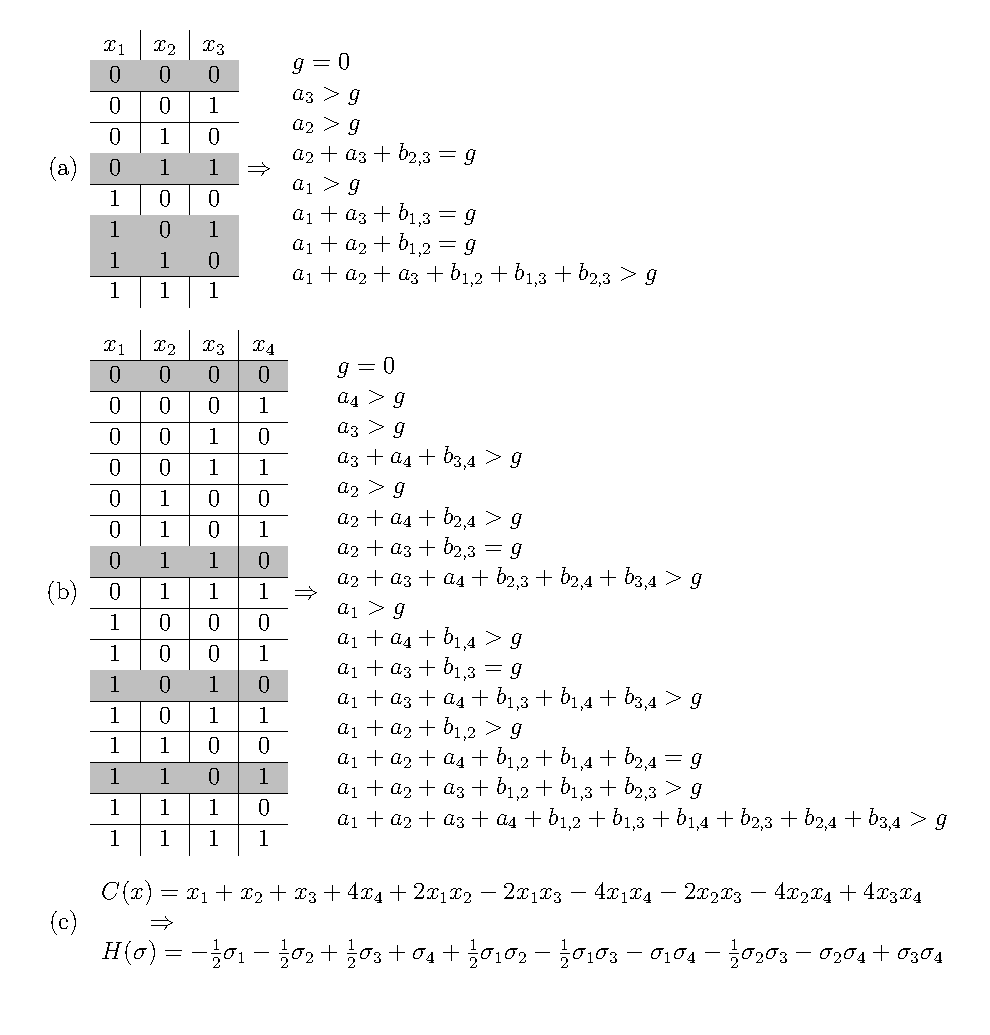
\includegraphics[width=0.9\textwidth]{fig2.pdf}
\caption{Embedding a quantum XOR gate: this figure illustrates the process of programming a quantum annealer, by embedding an XOR gate. The goal is to implement the circuit $x_1 \oplus x_2 = x_3$.
The truth table in (a) shows all combinations of $x_1$, $x_2$, and $x_3$, with all 4 valid input/output combinations highlighted.
Using the QUBO model, this generates the algebraic system of inequalities shown on the right hand side, where $g$ denotes the ground energy of the system.
Because the row containing all zeros is a valid solution, $g$ must be $0$.
The system of inequalities for (a) has no solution, so an ancillary bit $x_4$ is introduced in (b).
There are $2^4$ ways to assign the value of $x_4$ for the $4$ valid states from (a), some of which produce solvable systems and some of which do not.
By trial and error, the rows highlighted in (b) produce a solvable system, shown on the right hand side.
Solving this system produces the QUBO shown in (c), and applying the isomorphism results in the Hamiltonian below.
}
\label{fig:xor-ex}
\end{figure}